\documentclass[11pt,twocolumn]{article}
\usepackage[utf8]{inputenc}
\date{}

\usepackage{graphicx}
\usepackage{titlesec}
\usepackage{pgfplots}
\usepackage{listings}
\usepackage{subcaption}
\usepackage{amssymb}
\usepackage{amsmath}
\usepackage{float}
\usepackage{subfig}
\usepackage{subcaption}
\usepackage{pgfplots}
\usepackage{tikz}
\usepackage[font={small,it}]{caption}
\usepackage[top=0.5in, bottom=1in, left=1in, right=1.in]{geometry}
\usepackage{titlesec}
\usepackage[english]{babel}
\usepackage[utf8]{inputenc}

\usepackage[backend=biber]{biblatex}


\addbibresource{references.bib}


\titleformat*{\section}{\Large\bfseries}
\titleformat*{\subsection}{\large\bfseries}
\DeclareRobustCommand{\bbone}{\text{\usefont{U}{bbold}{m}{n}1}}
\DeclareMathOperator{\EX}{\mathbb{E}}



\begin{document}
\title{\centerline{\rule{15cm}{4pt}} \vspace*{0.2cm} \textbf{A Survey On Autoencoders}\vspace*{0.01cm} \\\centerline{\rule{15cm}{2pt}}}
\author{
  BILICI, M. Şafak\\
  \texttt{safakk.bilici.2112@gmail.com}}
\maketitle
\textbf{\textit{Abstract-}} \textbf{Autoencoders are an unsupervised learning architectures in neural networks. They are commonly used in Deep Learning tasks; such as generative models, anomaly detection, dimensionality reduction. In this article, we will evaluate theoretical approaches of Autoencoders and see it's extensions.}

\section{1 Introduction}
\hspace*{0.5cm} Autoencoders are an unsupervised learning method. They map the input data into lower dimensional space with encoder $E$, and then maps into same space that have same dimension of input data with decoder $D$.\\
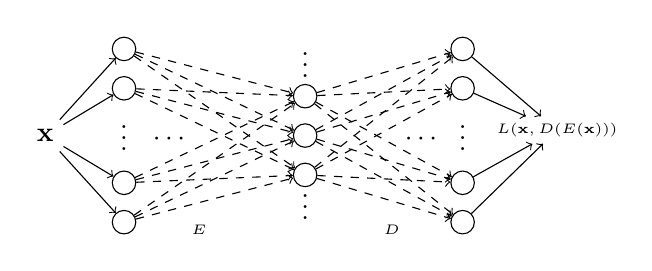
\begin{tikzpicture}

      \node[inner sep=3pt] (z) at (-0.4,-1.15){$\cdots$};
      \node[circle,draw=black,minimum size=0.2cm,inner sep=3pt] (a) at (-1,0){};
      \node[circle,draw=black,minimum size=0.1cm,inner sep=3pt] (b) at (-1,-0.5){};
      
      \node[] (e) at (0.2,0){};
      \node[circle,draw=black,minimum size=0.1cm,inner sep=3pt] (f) at (1.3,-0.6){};
      \node[circle,draw=black,minimum size=0.1cm,inner sep=3pt] (g) at (1.3,-1.1){};
      \node[circle,draw=black,minimum size=0.1cm,inner sep=3pt] (h) at (1.3,-1.6){};
      
      \node[inner sep=3pt] (z) at (-1,-1.03){$\vdots$};
     
      \node[circle,draw=black,minimum size=0.1cm,inner sep=3pt] (c) at (-1,-1.7){};
      \node[circle,draw=black,minimum size=0.1cm,inner sep=3pt] (d) at (-1,-2.2){};
      \node[] (w) at (-2,-1.1){$\mathbf{x}$};
      \node[inner sep=3pt] (o) at (2.8,-1.15){$\cdots$};
      \node[circle,draw=black,minimum size=0.2cm,inner sep=3pt] (i) at (3.3,0){};
      \node[circle,draw=black,minimum size=0.1cm,inner sep=3pt] (j) at (3.3,-0.5){};
      \node[inner sep=3pt] (m) at (3.3,-1.03){$\vdots$};
      \node[circle,draw=black,minimum size=0.1cm,inner sep=3pt] (k) at (3.3,-1.7){};
      \node[circle,draw=black,minimum size=0.1cm,inner sep=3pt] (l) at (3.3,-2.2){};
      
	  \node[inner sep=3pt] (m) at (1.3,-0.1){$\vdots$};      
	  \node[inner sep=3pt] (m) at (1.3,-1.9){$\vdots$};      
      
      
      \tiny
      \node[] (n) at (4.5,-1.03){$L(\mathbf{x},D(E(\mathbf{x})))$};
      
      \node[inner sep=3pt] (p) at (-0.05,-2.3){$E$};
      \node[inner sep=3pt] (r) at (2.4,-2.3){$D$};
      
      \draw[->] (w) -- (a);
      \draw[->] (w) -- (b);
      \draw[->] (w) -- (c);
      \draw[->] (w) -- (d);
      \draw[dashed,->] (a) -- (f);
      \draw[dashed,->] (a) -- (g);
      \draw[dashed,->] (a) -- (h);
      \draw[dashed,->] (b) -- (f);
      \draw[dashed,->] (b) -- (g);
      \draw[dashed,->] (b) -- (h);
      \draw[dashed,->] (c) -- (f);
      \draw[dashed,->] (c) -- (g);
      \draw[dashed,->] (c) -- (h);
      \draw[dashed,->] (d) -- (f);
      \draw[dashed,->] (d) -- (g);
      \draw[dashed,->] (d) -- (h);
      \draw[dashed,->] (f) -- (i);
      \draw[dashed,->] (f) -- (j);
      \draw[dashed,->] (f) -- (k);
      \draw[dashed,->] (f) -- (l);
      \draw[dashed,->] (g) -- (i);
      \draw[dashed,->] (g) -- (j);
      \draw[dashed,->] (g) -- (k);
      \draw[dashed,->] (g) -- (l);
      \draw[dashed,->] (h) -- (i);
      \draw[dashed,->] (h) -- (j);
      \draw[dashed,->] (h) -- (k);
      \draw[dashed,->] (h) -- (l);
      \draw[->] (i) -- (n);
      \draw[->] (j) -- (n);
      \draw[->] (k) -- (n);
      \draw[->] (l) -- (n);
    \end{tikzpicture}
The main idea behind Autoencoders is to attempt to copy its input to its output. The input layer is fed with input vector $\mathbf{x}$ and the loss is calculated at output layer between $\mathbf{x}$ and $E(D(\mathbf{x}))$, in other words the loss is $L(\mathbf{x},E(D(\mathbf{x})))$. It measures difference between our original input and the consequent reconstruction.  We named the middle layer, that is connection between encoder $E$ and decoder $D$, as the "bottleneck". We can denote our output of bottleneck as $\mathbf{h} = E(\mathbf{x})$ and denote our output as $\mathbf{\hat{x}} = D(\mathbf{h}) = D(E(\mathbf{x}))$. We can define our encoder and decoder as conditional probability density function that are $p_{encoder}(\mathbf{h} | \mathbf{x})$ and $p_{decoder}(\mathbf{\hat{x}} | \mathbf{h})$. \\
The loss function is named reconstruction loss which is $L(\mathbf{\hat{x}},\mathbf{x})$. We can treat the process as a feedforward networks; the loss can be minimized via mini-batch statistics following gradients computed by backpropagation algorithm,
\begin{equation}
\min\limits_{\theta} L = \nabla_\theta L(\mathbf{x}, D(E(\mathbf{x}))) =\nabla_\theta L(\mathbf{x}, \mathbf{\hat{x}})
\end{equation}
The bottleneck is the key of the effectiveness of Autoencoders. We map our input vector to bottleneck: the bottleneck keeps the 'latent informations' of input $\mathbf{x}$. The network represents input but in lower dimensions. In other words, it behaves like a approximative compression algorithm. The encoding parameters are learned in training process. Then we map bottleneck information $\mathbf{h}$ into same dimension as input $\mathbf{x}$. Then, this procedure can be seen as approximative extracting compressed latent information.

\section{2 Undercomplete Autoencoders}	
\hspace*{0.5cm} The simplest idea behind autoencoders is the decreasing the number of nodes through the hidden layers before bottleneck. An autoencoder that has dimension less than the input $\mathbf{x}$ is called undercomplete autoencoder. When we minimize the reconstruction error, autoencoder learns to represent latent attributes of input data with lower dimensions than input $\mathbf{x}$'s. This procedure is same as in Principal Component Analysis (PCA) but in non-linear way. When decoder is linear and the loss $L(\mathbf{\hat{x},\mathbf{x}})$ is the $L^2$ error, an autocomplete autoencoder learns to span the same subspace as PCA. When autoencoder has non-linear activations, then autoencoder becomes more powerful and generalized in dimensionality reduction, it becames non-linear version of PCA.
\begin{figure}[H]
\centering
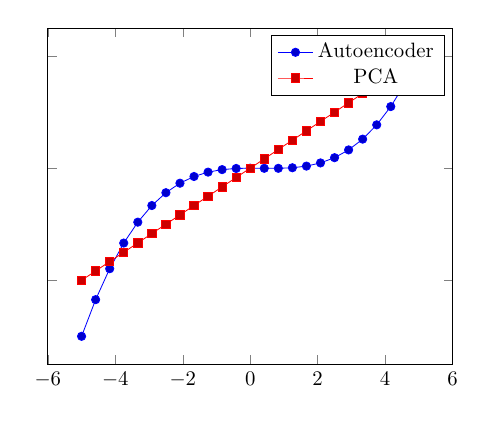
\begin{tikzpicture}[scale=0.75]
  \begin{axis}[%
      title={},
      xlabel={},
      ylabel={},
      yticklabels={,,}
    ]
    \addplot {x^3 - x^2 }; 
    \addplot { 20 * x};
    \addlegendentry{Autoencoder}
	\addlegendentry{PCA}
  \end{axis}
\end{tikzpicture}
\caption{Encoding of PCA and Autoencoder.}
\end{figure}
\subsection{2.1 Problem of Autoencoders}
When we said that main idea behind autoencoders is to copy input to its output, the key idea is that not to copy without extracting useful informations about the distribution of the data \cite{Goodfellow-et-al-2016}. Autoencoders are allowed too much capacity, easy to be trained to the copying the task with learning anything useful about the dataset. So we need to penalize those autoencoders.

\section{3 Regularizations}
As we said, autoencoders are allowerd too much capacity. Regularized autoencoders can give us the task that find the latent features of input, instead of copying the input. There are lot of regularization methods to prevent copying task such as Sparse Autoencoders or Denoising Autoencoders. 

\subsection{3.1 Denoising Autoencoders}
We can achieve the task that learning useful informations about data by adding some noise to input data. 
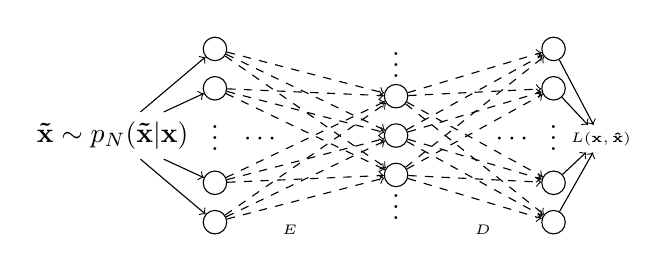
\begin{tikzpicture}

      \node[inner sep=3pt] (z) at (-0.4,-1.15){$\cdots$};
      \node[circle,draw=black,minimum size=0.2cm,inner sep=3pt] (a) at (-1,0){};
      \node[circle,draw=black,minimum size=0.1cm,inner sep=3pt] (b) at (-1,-0.5){};
      
      \node[] (e) at (0.2,0){};
      \node[circle,draw=black,minimum size=0.1cm,inner sep=3pt] (f) at (1.3,-0.6){};
      \node[circle,draw=black,minimum size=0.1cm,inner sep=3pt] (g) at (1.3,-1.1){};
      \node[circle,draw=black,minimum size=0.1cm,inner sep=3pt] (h) at (1.3,-1.6){};
      
      \node[inner sep=3pt] (z) at (-1,-1.03){$\vdots$};
     
      \node[circle,draw=black,minimum size=0.1cm,inner sep=3pt] (c) at (-1,-1.7){};
      \node[circle,draw=black,minimum size=0.1cm,inner sep=3pt] (d) at (-1,-2.2){};
      \node[] (w) at (-2.3,-1.1){$\mathbf{\tilde{x}} \sim p_{N}(\mathbf{\tilde{x}}|\mathbf{x})$};
      \node[inner sep=3pt] (o) at (2.8,-1.15){$\cdots$};
      \node[circle,draw=black,minimum size=0.2cm,inner sep=3pt] (i) at (3.3,0){};
      \node[circle,draw=black,minimum size=0.1cm,inner sep=3pt] (j) at (3.3,-0.5){};
      \node[inner sep=3pt] (m) at (3.3,-1.03){$\vdots$};
      \node[circle,draw=black,minimum size=0.1cm,inner sep=3pt] (k) at (3.3,-1.7){};
      \node[circle,draw=black,minimum size=0.1cm,inner sep=3pt] (l) at (3.3,-2.2){};
      
	  \node[inner sep=3pt] (m) at (1.3,-0.1){$\vdots$};      
	  \node[inner sep=3pt] (m) at (1.3,-1.9){$\vdots$};      
      
      
      \tiny
      \node[] (n) at (3.9,-1.14){$L(\mathbf{x},\mathbf{\hat{x}})$};
      
      \node[inner sep=3pt] (p) at (-0.05,-2.3){$E$};
      \node[inner sep=3pt] (r) at (2.4,-2.3){$D$};
      
      \draw[->] (w) -- (a);
      \draw[->] (w) -- (b);
      \draw[->] (w) -- (c);
      \draw[->] (w) -- (d);
      \draw[dashed,->] (a) -- (f);
      \draw[dashed,->] (a) -- (g);
      \draw[dashed,->] (a) -- (h);
      \draw[dashed,->] (b) -- (f);
      \draw[dashed,->] (b) -- (g);
      \draw[dashed,->] (b) -- (h);
      \draw[dashed,->] (c) -- (f);
      \draw[dashed,->] (c) -- (g);
      \draw[dashed,->] (c) -- (h);
      \draw[dashed,->] (d) -- (f);
      \draw[dashed,->] (d) -- (g);
      \draw[dashed,->] (d) -- (h);
      \draw[dashed,->] (f) -- (i);
      \draw[dashed,->] (f) -- (j);
      \draw[dashed,->] (f) -- (k);
      \draw[dashed,->] (f) -- (l);
      \draw[dashed,->] (g) -- (i);
      \draw[dashed,->] (g) -- (j);
      \draw[dashed,->] (g) -- (k);
      \draw[dashed,->] (g) -- (l);
      \draw[dashed,->] (h) -- (i);
      \draw[dashed,->] (h) -- (j);
      \draw[dashed,->] (h) -- (k);
      \draw[dashed,->] (h) -- (l);
      \draw[->] (i) -- (n);
      \draw[->] (j) -- (n);
      \draw[->] (k) -- (n);
      \draw[->] (l) -- (n);
    \end{tikzpicture}
In other words, we can achive it by changing the reconstruction loss. We defined our minimization,
\begin{equation}
\min\limits_{\theta} L = \nabla_\theta L(\mathbf{x}, D(E(\mathbf{x}))) =\nabla_\theta L(\mathbf{x}, \mathbf{\hat{x}})
\end{equation}
To perform the denoising, the input $\mathbf{x}$ is corrupted into $\mathbf{\tilde{x}}$ through stochastic mapping  of $\mathbf{\tilde{x}} \sim p_{N}(\mathbf{\tilde{x}}|\mathbf{x})$. Then the noisy (corrupted) input is used for encoding and decoding parts
\begin{equation}
\mathbf{h} = E(\mathbf{\tilde{x}})
\end{equation}
\begin{equation}
\mathbf{\hat{x}} = D(\mathbf{h}) = D(E(\mathbf{\tilde{x}})_{\mathbf{\tilde{x}} \sim p_{N}(\mathbf{\tilde{x}}|\mathbf{x})})
\end{equation}
Then the minimization task is updated as 
\begin{equation}
\min\limits_{\theta} L = \nabla_\theta L(\mathbf{x}, D(E(\mathbf{\tilde{x}})_{\mathbf{\tilde{x}} \sim p_{N}(\mathbf{\tilde{x}}|x)})) =\nabla_\theta L(\mathbf{x}, \mathbf{\hat{x}}) 
\end{equation}
The denoising can be seen as forcing our model to learn latent features of our input by adding noise to input then penalizing with reconstruction loss $L(\mathbf{x}, \mathbf{\hat{x}})$.
\subsection{Sparse Autoencoders}
The sparsity simply comes from adding a shrinkage method to reconstruction loss like in machine learning tasks.
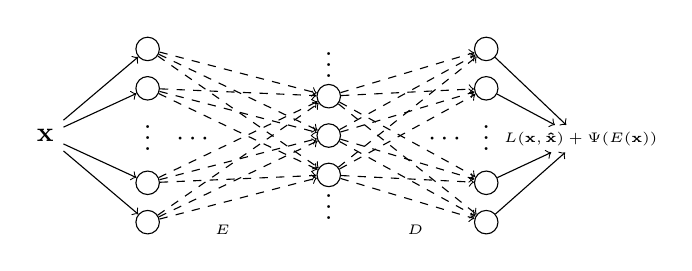
\begin{tikzpicture}

      \node[inner sep=3pt] (z) at (-0.4,-1.15){$\cdots$};
      \node[circle,draw=black,minimum size=0.2cm,inner sep=3pt] (a) at (-1,0){};
      \node[circle,draw=black,minimum size=0.1cm,inner sep=3pt] (b) at (-1,-0.5){};
      
      \node[] (e) at (0.2,0){};
      \node[circle,draw=black,minimum size=0.1cm,inner sep=3pt] (f) at (1.3,-0.6){};
      \node[circle,draw=black,minimum size=0.1cm,inner sep=3pt] (g) at (1.3,-1.1){};
      \node[circle,draw=black,minimum size=0.1cm,inner sep=3pt] (h) at (1.3,-1.6){};
      
      \node[inner sep=3pt] (z) at (-1,-1.03){$\vdots$};
     
      \node[circle,draw=black,minimum size=0.1cm,inner sep=3pt] (c) at (-1,-1.7){};
      \node[circle,draw=black,minimum size=0.1cm,inner sep=3pt] (d) at (-1,-2.2){};
      \node[] (w) at (-2.3,-1.1){$\mathbf{x}$};
      \node[inner sep=3pt] (o) at (2.8,-1.15){$\cdots$};
      \node[circle,draw=black,minimum size=0.2cm,inner sep=3pt] (i) at (3.3,0){};
      \node[circle,draw=black,minimum size=0.1cm,inner sep=3pt] (j) at (3.3,-0.5){};
      \node[inner sep=3pt] (m) at (3.3,-1.03){$\vdots$};
      \node[circle,draw=black,minimum size=0.1cm,inner sep=3pt] (k) at (3.3,-1.7){};
      \node[circle,draw=black,minimum size=0.1cm,inner sep=3pt] (l) at (3.3,-2.2){};
      
	  \node[inner sep=3pt] (m) at (1.3,-0.1){$\vdots$};      
	  \node[inner sep=3pt] (m) at (1.3,-1.9){$\vdots$};      
      
      
      \tiny
      \node[] (n) at (4.5,-1.14){$L(\mathbf{x},\mathbf{\hat{x}})+\Psi(E(\mathbf{x}))$};
      
      \node[inner sep=3pt] (p) at (-0.05,-2.3){$E$};
      \node[inner sep=3pt] (r) at (2.4,-2.3){$D$};
      
     
      
      \draw[->] (w) -- (a);
      \draw[->] (w) -- (b);
      \draw[->] (w) -- (c);
      \draw[->] (w) -- (d);
      \draw[dashed,->] (a) -- (f);
      \draw[dashed,->] (a) -- (g);
      \draw[dashed,->] (a) -- (h);
      \draw[dashed,->] (b) -- (f);
      \draw[dashed,->] (b) -- (g);
      \draw[dashed,->] (b) -- (h);
      \draw[dashed,->] (c) -- (f);
      \draw[dashed,->] (c) -- (g);
      \draw[dashed,->] (c) -- (h);
      \draw[dashed,->] (d) -- (f);
      \draw[dashed,->] (d) -- (g);
      \draw[dashed,->] (d) -- (h);
      \draw[dashed,->] (f) -- (i);
      \draw[dashed,->] (f) -- (j);
      \draw[dashed,->] (f) -- (k);
      \draw[dashed,->] (f) -- (l);
      \draw[dashed,->] (g) -- (i);
      \draw[dashed,->] (g) -- (j);
      \draw[dashed,->] (g) -- (k);
      \draw[dashed,->] (g) -- (l);
      \draw[dashed,->] (h) -- (i);
      \draw[dashed,->] (h) -- (j);
      \draw[dashed,->] (h) -- (k);
      \draw[dashed,->] (h) -- (l);
      \draw[->] (i) -- (n);
      \draw[->] (j) -- (n);
      \draw[->] (k) -- (n);
      \draw[->] (l) -- (n);
    \end{tikzpicture}\\
The minimization will be
\begin{equation}
\min\limits_{\theta} L = \nabla_\theta L(\mathbf{x}, D(E(\mathbf{x}))) + \underbrace{\Psi(E(\mathbf{x}))}_{\text sparisty} =\nabla_\theta L(\mathbf{x}, \mathbf{\hat{x}}) 
\end{equation}
This procedure can be interpreted as Bayesian inference with terms of posterior, likelihood and prior: $posterior \propto likelihood \times prior$. From this point maximizing the likelihood is equivalent to maximizing the posterior
\begin{equation}
\max\limits_{\theta} p(\theta,\mathbf{x})=\max\limits_{\theta} p(\mathbf{x},\theta) \cdot p(\theta)
\end{equation}
\begin{equation}
=\max\limits_{\theta}\log p(\mathbf{x} | \theta) + \log p(\theta)
\end{equation}
Now we can write our joint distribution in terms of prior of $\mathbf{h}$ and it's factor seeing  $\mathbf{x}$ 
\begin{equation}
p_{model}(\mathbf{x},\mathbf{h}) = p_{model}(\mathbf{x}|\mathbf{h}) \cdot p_{model}(\mathbf{h})
\end{equation}
From this point, we can rewrite our likelihood and propose a prior distribution.
\begin{equation} 
\log p_{model}(\mathbf{x},\mathbf{h}) = \log p_{model}(\mathbf{x}|\mathbf{h}) + \log p_{model}(\mathbf{h})
\end{equation}
For simplicity, let us consider a zero-mean Laplacean prior \cite{Goodfellow-et-al-2016}
\begin{equation} 
Lap(h_i|\mu=0,\lambda) = \frac{\lambda}{2}\exp(-\lambda|h_i - \mu|)
\end{equation}
\begin{equation} 
 = \frac{\lambda}{2}\exp(-\lambda|h_i |)
\end{equation}
Then the posterior becomes
\begin{equation} 
\prod p_{model}(\mathbf{x}|h) \cdot \prod  p_{model}(h)
\end{equation}
\begin{equation} 
= \sum \log p_{model}(\mathbf{x}|h) + \sum \log  p_{model}(h)
\end{equation}
\begin{equation}
 = \sum \log p_{model}(\mathbf{x}|h) - \lambda \sum |h|
\end{equation}
Other prior distributions like Student-t or Gaussian ($\text{L}_1$)  can make an impact for sparsity \cite{Goodfellow-et-al-2016}.
\section{4 Variational Autoencoders}

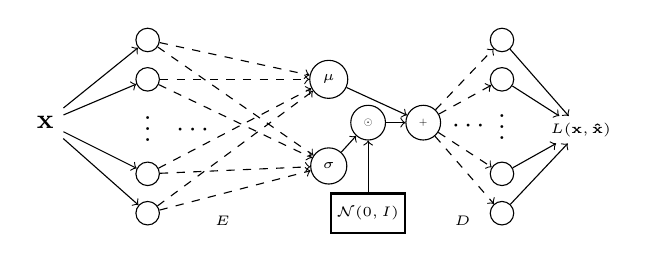
\begin{tikzpicture}
      \node[inner sep=3pt] (z) at (-0.4,-1.15){$\cdots$};
      \node[circle,draw=black,minimum size=0.2cm,inner sep=3pt] (a) at (-1,0){};
      \node[circle,draw=black,minimum size=0.1cm,inner sep=3pt] (b) at (-1,-0.5){};
      
      \node[] (e) at (0.2,0){};
      \node[circle,draw=black,minimum size=0.1cm,inner sep=3pt] (f) at (1.3,-0.5){\tiny $\mu$};
      \node[circle,draw=black,minimum size=0.1cm,inner sep=3pt] (g) at (1.3,-1.6){\tiny$\sigma$};
      
       \node[circle,draw=black,minimum size=0.1cm,inner sep=3pt] (q) at (1.8,-1.05){ \scalebox{.4}{$\odot$}};
        \node[circle,draw=black,minimum size=0.1cm,inner sep=3pt] (y) at (2.5,-1.05){ \scalebox{.4}{$+$}};
        
      %\node[circle,draw=black,minimum size=0.1cm,inner sep=3pt] (h) at (1.3,-1.6){};
      
      \node[inner sep=3pt] (z) at (-1,-1.03){$\vdots$};
     
      \node[circle,draw=black,minimum size=0.1cm,inner sep=3pt] (c) at (-1,-1.7){};
      \node[circle,draw=black,minimum size=0.1cm,inner sep=3pt] (d) at (-1,-2.2){};
      \node[] (w) at (-2.3,-1.05){$\mathbf{x}$};
      \node[inner sep=3pt] (o) at (3.1,-1.1){$\cdots$};
      \node[circle,draw=black,minimum size=0.2cm,inner sep=3pt] (i) at (3.5,0){};
      \node[circle,draw=black,minimum size=0.1cm,inner sep=3pt] (j) at (3.5,-0.5){};
      \node[inner sep=3pt] (m) at (3.5,-1.0){$\vdots$};
      \node[circle,draw=black,minimum size=0.1cm,inner sep=3pt] (k) at (3.5,-1.7){};
      \node[circle,draw=black,minimum size=0.1cm,inner sep=3pt] (l) at (3.5,-2.2){};
      
	  %\node[inner sep=3pt] (m) at (1.3,-0.1){$\vdots$};      
	  %\node[inner sep=3pt] (m) at (1.3,-1.9){$\vdots$};      
      
      
      \tiny
      \node[] (n) at (4.5,-1.14){$L(\mathbf{x},\mathbf{\hat{x}})$};
      
      \node[inner sep=3pt] (p) at (-0.05,-2.3){$E$};
      \node[inner sep=3pt] (r) at (3,-2.3){$D$};
      
	    
      
      
      \draw[->] (w) -- (a);
      \draw[->] (w) -- (b);
      \draw[->] (w) -- (c);
      \draw[->] (w) -- (d);
      \draw[dashed,->] (a) -- (f);
      \draw[dashed,->] (a) -- (g);
      %\draw[dashed,->] (a) -- (h);
      \draw[dashed,->] (b) -- (f);
      \draw[dashed,->] (b) -- (g);
      %\draw[dashed,->] (b) -- (h);
      \draw[dashed,->] (c) -- (f);
      \draw[dashed,->] (c) -- (g);
      %\draw[dashed,->] (c) -- (h);
      \draw[dashed,->] (d) -- (f);
      \draw[dashed,->] (d) -- (g);
      %\draw[dashed,->] (d) -- (h);
      %\draw[dashed,->] (f) -- (i);
      %\draw[dashed,->] (f) -- (j);
      %\draw[dashed,->] (f) -- (k);
      %\draw[dashed,->] (f) -- (l);
      %\draw[dashed,->] (g) -- (i);
      %\draw[dashed,->] (g) -- (j);
      %\draw[dashed,->] (g) -- (k);
      %\draw[dashed,->] (g) -- (l);
      %\draw[dashed,->] (h) -- (i);
      %\draw[dashed,->] (h) -- (j);
      %\draw[dashed,->] (h) -- (k);
      %\draw[dashed,->] (h) -- (l);
       \node (rect) at (1.80,-2.2) [draw,thick,minimum width=0.5cm,minimum height=0.5cm] {$\mathcal{N}(0,I)$};
      \draw[->] (i) -- (n);
      \draw[->] (j) -- (n);
      \draw[->] (k) -- (n);
      \draw[->] (l) -- (n);
      \draw[->] (f) -- (y);
      \draw[->] (g) -- (q);
      \draw[->] (q) -- (y);
      \draw[dashed,->] (y) -- (i);
      \draw[dashed,->] (y) -- (j);
      \draw[dashed,->] (y) -- (k);
      \draw[dashed,->] (y) -- (l);
      \draw[->] (rect) -- (q);
    \end{tikzpicture}\\
\hspace*{0.5cm} Generative models are one of the main research area of Deep Learning for last decade. Variational Autoencoders are generative models. Variational Autoencoders perform efficient approximate inference and learning with directed probabilistic models whose continuous latent variables and/or parameters have intractable prior distributions \cite{kingma2014autoencoding}. 
\subsection{4.1 Latent Space Models}
\hspace*{0.5cm} Let's define our prior distribution. Our dataset is sampled form $x \sim p(X)$ and the latent variable is sampled from $z \sim p(Z)$. If we define our deterministic neural network as $f: Z \times \Theta \rightarrow X$ \cite{doersch2016tutorial}, ($\Theta$ is our parameter space), then $p(X)$ will be
\begin{equation} 
p(X) = \int p(X|z;\theta)p(z)dz
\end{equation} 
where $p(X|z;\theta)$ is another form of our deterministic neural network function.
\subsection{4.2 Setting Up The Objective}
\hspace*{0.5cm}Let's define $q_\phi(z|x)$ as our probabilistic encoder. It represents, the probability of $z$ when $x$ is known. Second, $p_\theta(x|z)$ as our probabilistic decoder. It represents, the probability of $x$ when $z$ is known \cite{kingma2014autoencoding}. The motivation behind Variational Autoencoders is to produce a output distribution which is equivalent (good reconstructing) to the input distribution. This task can be achieved with Kullback-Leibler Divergence defined as 
\begin{equation} 
D_{KL}(p||q) = \int_x p(x) \log \frac{p(x)}{q(x)}
\end{equation} 
\begin{equation} 
= \mathbb{E}[\log p(x) - \log q(x)]
\end{equation} 
The output distribution has a prior on $z$, which makes our true posterior as 
\begin{equation} 
p(z|x) = \frac{p(x|z) p(z)}{\int p(x|z)p(z) dz} = \frac{p(x|z) p(z)}{p(x)}
\end{equation} 
\begin{equation}
= \log p(z|x) = \log p(x|z) + \log p(z) - \log p(x)
\end{equation} 
From this point of view KL-Divergence of the approximate from the true posterior will be defined as 
\begin{equation}
D_{KL}(q_\phi(z|x^{(i)}) || p_\theta(z|x^{(i)}))
\end{equation} 
\begin{equation}
= \mathbb{E}_{q_\phi(z|x)}[\log q_\phi(z|x^{(i)}) - \log p_\theta(z|x^{(i)})]
\end{equation} 
$$ = \mathbb{E}_{q_\phi(z|x)}[\log q_\phi(z|x^{(i)}) - \log p(x^{(i)}|z) - \log p(z)]$$
\begin{equation}
\qquad \qquad \qquad \qquad \qquad \qquad \qquad + \log x^{(i)}
\end{equation} 
Putting Equation 21 and Equation 23 together simplifies,
\begin{equation}
\log p_\theta(x^{(i)}) - D_{KL}(q_\phi(z|x^{(i)}) || p_\theta(z|x^{(i)}))
\end{equation} 
\begin{equation}
=D_{KL}(q_\phi(z|x^{(i)}) || p_\theta(z)) - \mathbb{E}_{q_\phi(z|x^{(i)})}[\log p_\theta (x^{(i)}|z)]
\end{equation} 
Where Equation 25 references variational lower bound $\mathcal{L}(\theta,\phi;x^{(i)})$ \cite{kingma2014autoencoding} \cite{cs228} which is $\log p(x^{(i)}) \geq \mathcal{L}(\theta,\phi;x^{(i)})$. We want to differentiate and optimize this lower bound both on decoder parameters $\theta$ and encoder parameters $\phi$.

\printbibliography[title=References]

\end{document}